 \documentclass{homeworg}
\usepackage{amsmath}

\title{Travail 6 - Circuits digitaux CMOS}
\author{Wats Raphaël}

\begin{document}
\maketitle

\section{La fonction logique}
\begin{center}
\huge
$AC + A'B$\\
\end{center}

\section{La table de vérité de la fonction logique}
\begin{center}
    \huge
    \begin{tabular}{|l|c|r|r|}
      \hline
      A & B & C & Y\\
      \hline
      0 & 0 & 0 & 0\\
      0 & 0 & 1 & 0\\
      0 & 1 & 0 & 1\\
      0 & 1 & 1 & 1\\
      1 & 0 & 0 & 0\\
      1 & 0 & 1 & 1\\
      1 & 1 & 0 & 0\\
      1 & 1 & 1 & 1\\
      \hline
    \end{tabular}
\end{center}

\newpage
\section{Le schéma du circuit CMOS avec le dimensionnement des transistors}
    \begin{center}
        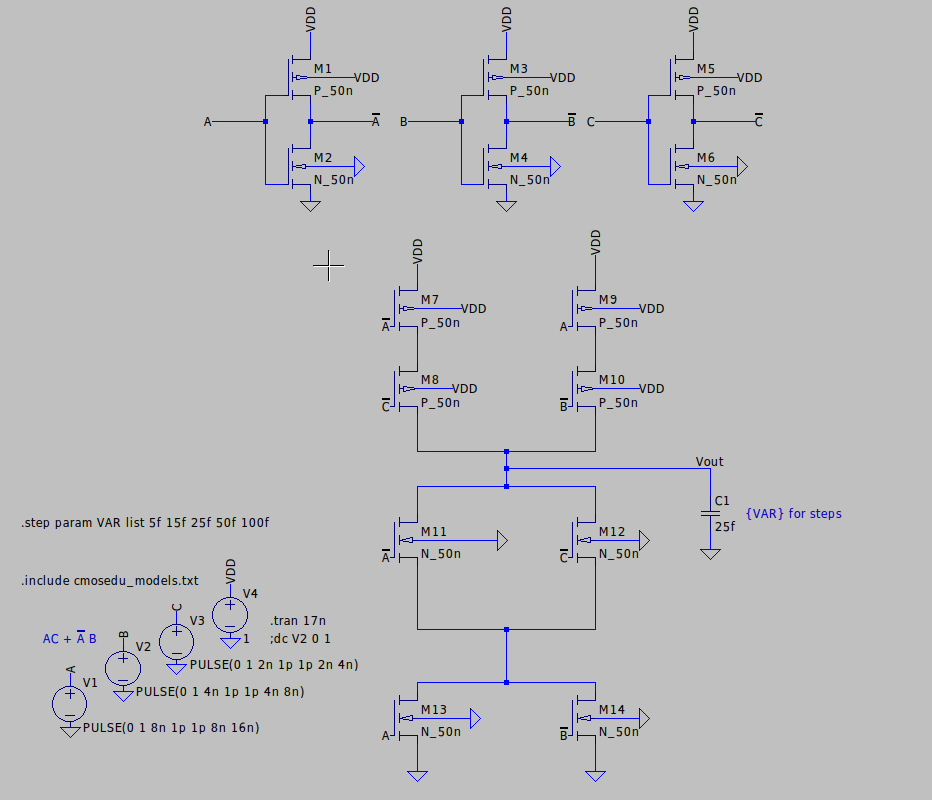
\includegraphics[scale=0.6]{circuit.png}\\
    \end{center}
    Pour commencer les voltages A, B et C parcourrent dans l'ordre les différentes combinaisons possibles de la table de vérité. Un circuit CMOS est composé de deux types de transistors ici le standard est 50nm pour la longueur:
    \begin{itemize}
        \item Les transistors PMOS ont alors pour largeur le nombre de PMOS en série * $1\mu m$.
        \item Les transistors NMOS ont alors pour largeur le nombre de NMOS en série * $500nm$.
    \end{itemize}
    
     Par exemple:
     \begin{itemize}
         \item Le transistor PMOS M1, M3 et M5 ont $50nm$ de longueur et $1\mu m$ de largeur.
         \item Le transistor NMOS M2, M4 et M6 ont $50nm$ de longueur et $500nm$ de largeur.
         \item Les transistors PMOS M7, M8, M9 et M10 ont tous $50nm$ de longueur et $2\mu m$
         \item Les transistors NMOS M11, M12, M13, M14 ont tous $50nm$ de longueur et $1\mu m$
     \end{itemize}
     La longueur bien que plus petite que la largeur s'apelle ainsi car elle décrit en réalité la vitesse à laquelle le transistor opère.
     \newpage
     
     La partie supérieur PMOS du circuit représente la fonction logique implémentée où les transistors en série représente une opération AND et les transistors en paralèle représente une opération OR. Comme un transistor PMOS ne laisse pas le voltage haut VDD passé lorsque l'entrée est à tension haute et inversément on doit cependant inversée les entrées de la fonction logique. La partie inférieur NMOS du circuit représente la fonction logique inverse (obtenu grâce à la loi de De Morgan).
     
     Enfin le C de CMOS signifie Complémentaire car l'on a besoin d'une partie PMOS bonne à transmettre un haut voltage mais pas à transmettre un voltage faible ainsi à l'inverse la partie NMOS bonne à transmettre un voltage faible mais pas à transmettre un voltage élevé.\\[1cm]

\section{La simulation .dc en faisant varier une des entrées de 0 à 1V}
    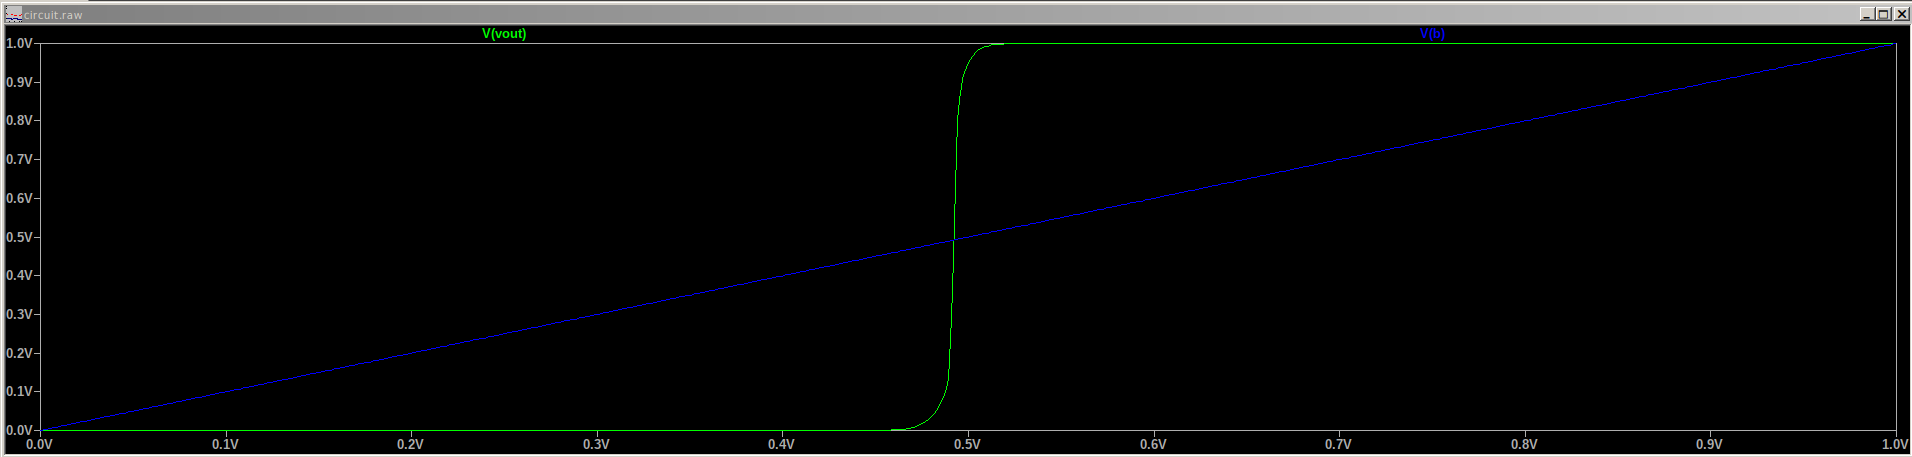
\includegraphics[scale=0.3]{dc.png}\\[1cm]

\section{La simulation .tran en faisant varier une des entrées et en faisant varier la capacité de sorties}
    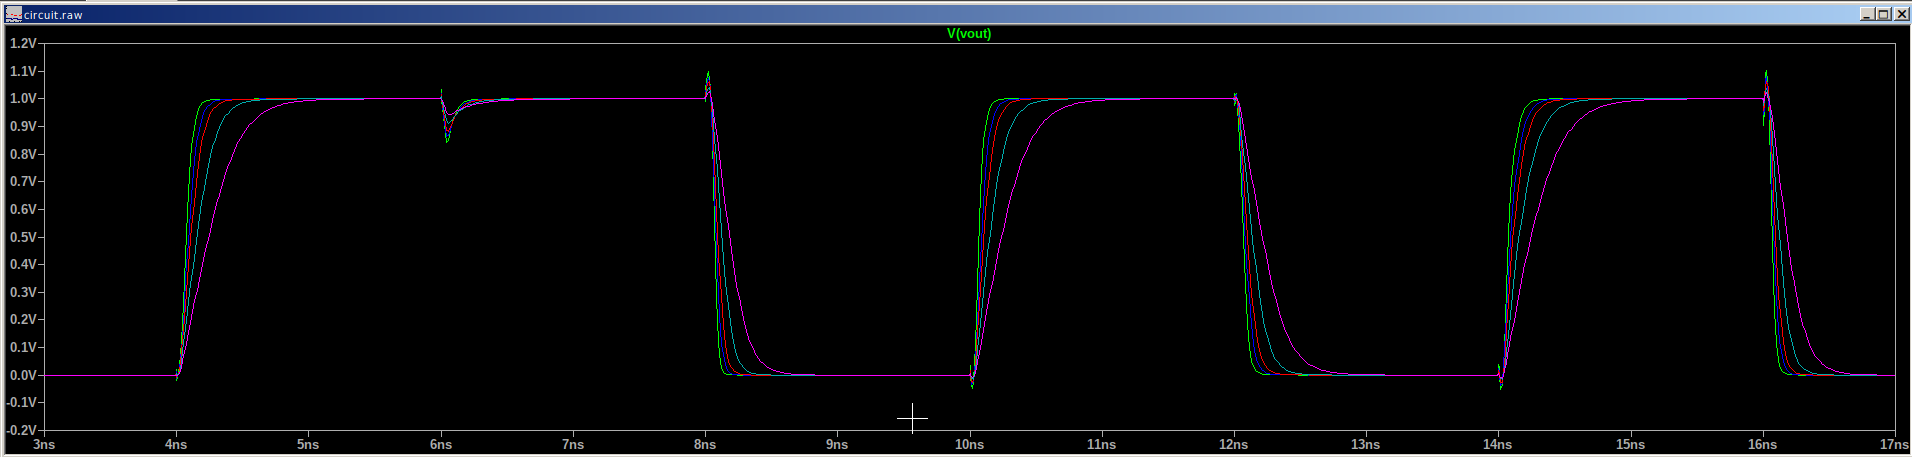
\includegraphics[scale=0.3]{capa.png}
\section{La simulation .tran en faisant varier les 3 entrées de manière à parcourir la table de vérité de la fonction}
    \begin{center}
        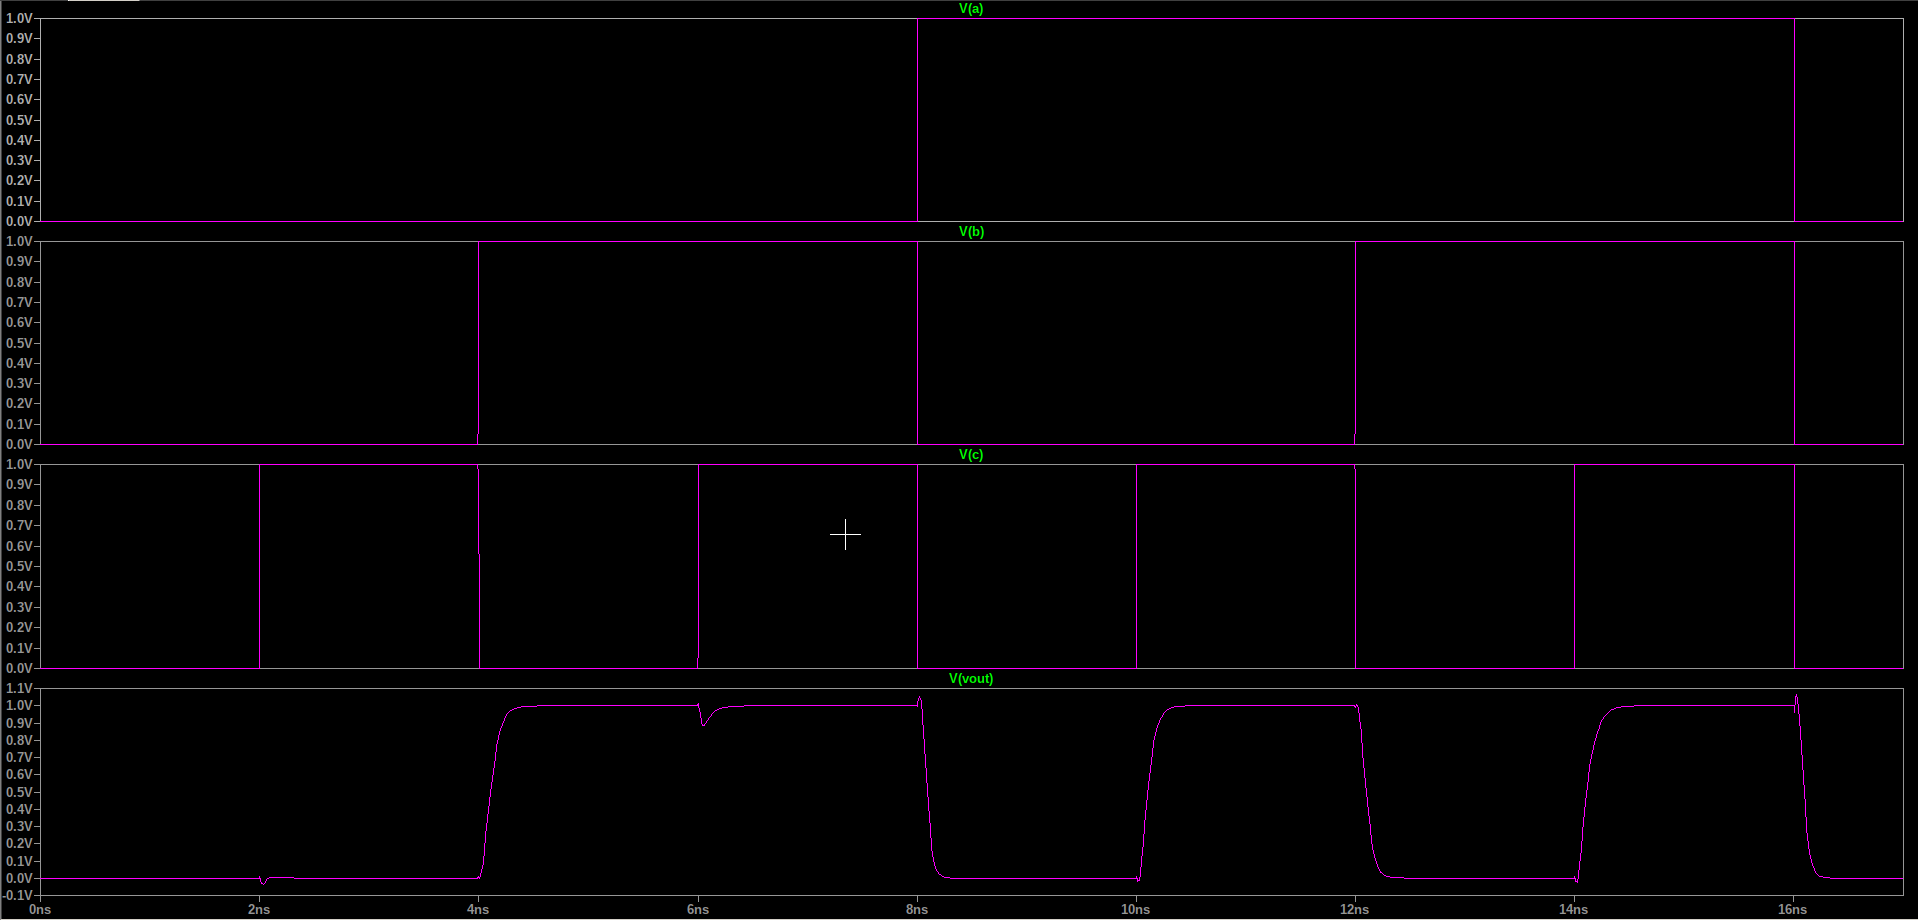
\includegraphics[scale=0.3]{plot.png}
    \end{center}

\section{Conclusion}
    Les résultats obtenu sont en adéquation avec ceux obtenu lors des simulations LTspice XVII.
    \begin{itemize}
        \item Grâce aux transistors nous pouvons construire des circuit logiques de plus en plus complexes
    \end{itemize}
\end{document}
